\documentclass[UTF8,fontset=none,11pt]{ctexart}
\usepackage[a4paper,margin=22mm]{geometry}
\usepackage{fontspec,graphicx,booktabs,xcolor,hyperref,fancyhdr,float,needspace}
\setCJKmainfont{Songti SC}\setCJKsansfont{Heiti SC}\setCJKmonofont{Heiti SC}
\setmainfont{Times New Roman}\setsansfont{Arial}\setmonofont{Menlo}
\definecolor{NeutralBlue}{HTML}{2878B5}\definecolor{BoidsOrange}{HTML}{D97932}
\definecolor{IndependentGray}{HTML}{737C86}\definecolor{TextInk}{HTML}{243544}
\hypersetup{colorlinks=true,linkcolor=NeutralBlue,urlcolor=NeutralBlue}
\ctexset{section={format=\Large\sffamily\bfseries\color{TextInk}}}
\pagestyle{fancy}\fancyhf{}\fancyhead[L]{\small Boids 工具生态：冻结数据分析}\fancyhead[R]{\small 2026-10-09}\fancyfoot[C]{\thepage}
\setlength{\headheight}{15pt}\setlength{\parskip}{5pt}\linespread{1.18}
\setcounter{topnumber}{3}\renewcommand{\topfraction}{.9}\renewcommand{\textfraction}{.08}
\begin{document}
\title{Boids 工具生态：从复用到分工，究竟走到了哪一步？}\author{现有数据分析工作稿}\date{2026年10月9日}\maketitle
本稿只分析已经完成的九个社会。新增模型调用为零，新增 grader 调用为零，不执行生成工具，不追加任务、干预或修复。所有数字来自冻结公开档案及此前完成的共同面板审计。原始成绩、失败记录和生成版本不变。

\textbf{核心判断：局部 Boids 提示下，实际工具采用更多，作者维护能力的依赖结构不同；稳定、必要的互补分工没有被这批任务验证出来。} 这两个判断可以同时成立。

\section{先把“合作成功”拆开}
设想八个同学做数据分析工具。一个同学写了完整工具箱，其他人开始使用。我们至少能问四个不同的问题：别人是否真的用了它；它是否影响了计算结果；大家是否形成持续而不同的贡献；八个人合在一起是否获得一个人没有的能力。

前两个问题主要研究传播和功能依赖，后两个才接近互补分工。把别人的整套工具箱转发出来，可以是一项真实、有用的采用行为，但不能单凭转发就认定八个人形成了八个互补专业。反过来，最终覆盖没有提升，也不能抹去已经发生的实际采用。

\begin{figure}[H]\centering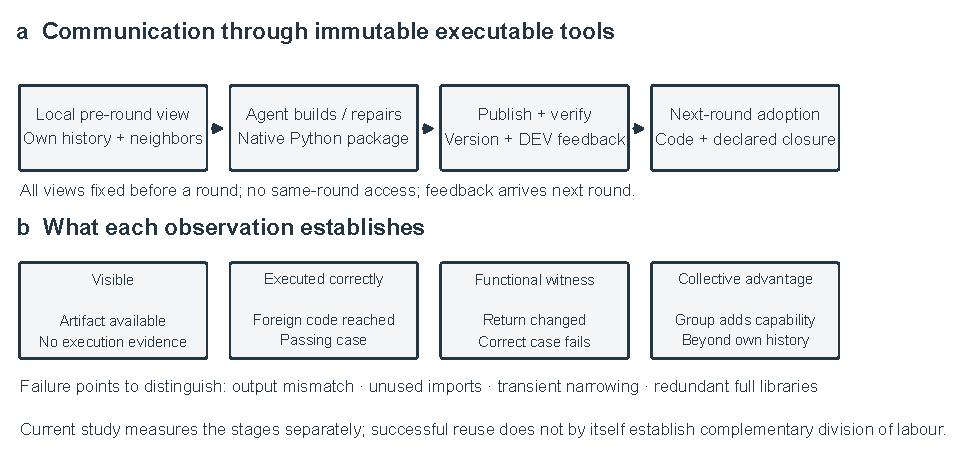
\includegraphics[width=\textwidth]{../../studies/tool_ecology/evidence/v031/analysis-02/figures/fig01-tool-communication.pdf}\caption{工具通信与证据层级}\end{figure}
\section{本轮到底研究什么}
每个社会八个 agent、六轮，没有预分配角色。所有人面对相同六类持续需求：清洗、收入计算、分组、月度汇总、目标比值和滚动均值。下游确实需要上游生成的新值，例如标准化地区和收入，不是把互不相干的函数摆在一起。

三种条件分别是局部中性、局部 Boids 和独立生成后合库，每种三个种子。局部组通过固定 ring 接收邻居工具及声明依赖闭包。独立组只看自己的历史。所有人读轮前快照，不能看到同轮新工具；下一轮才获得发布和 DEV 反馈。

这里的 Boids 是三条方向性提示。S 鼓励避免不必要的重复建设；A 鼓励复用经过验证的邻居接口；C 鼓励贴合持续需求和邻居近期能力。三条一起启用，没有分开估计。中性组也允许复用、修复和专业化，因此对比不是“允许合作”与“禁止合作”。

\begin{figure}[H]\centering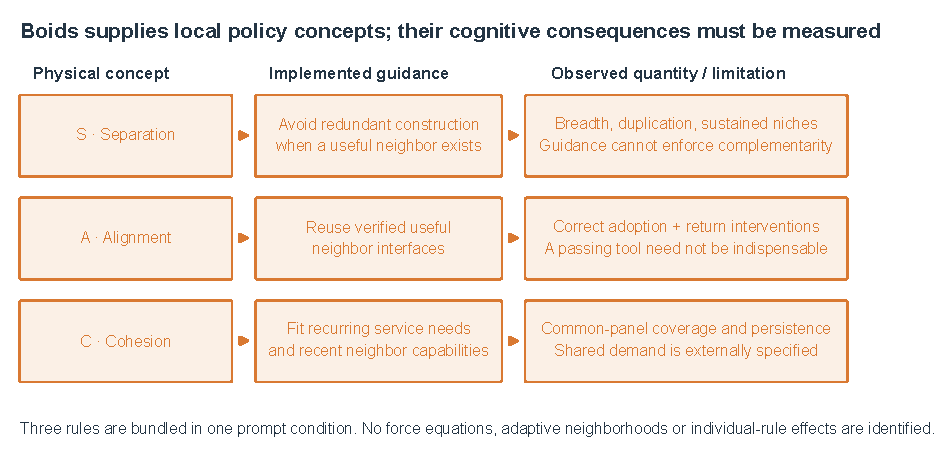
\includegraphics[width=\textwidth]{../../studies/tool_ecology/evidence/v031/analysis-02/figures/fig02-boids-mapping.pdf}\caption{当前 Boids 映射}\end{figure}
这是受控的探索性机制研究。它不是外部 benchmark 排名，不是原始物理 Boids 的数值复现，也没有完成持续单 agent 或集中分工的付费对照。

\Needspace{18\baselineskip}
\section{全部九个社会的大表}
下表单独保存为 \href{https://github.com/xisen-w/boids-evolution/blob/codex/tool-ecology-dynamics/studies/tool_ecology/evidence/v031/analysis-02/all-societies.md}{逐种子大表}，机器可读完整版是 \href{https://github.com/xisen-w/boids-evolution/blob/codex/tool-ecology-dynamics/studies/tool_ecology/evidence/v031/analysis-02/societies.csv}{societies.csv}。

\begin{center}\small\resizebox{\textwidth}{!}{\begin{tabular}{llllllllll}\toprule
种子 & 条件 & 发布/48 & 全六类 & 采用/后首轮 & 采用率 & 跨作者案例 & 自足六类/8 & 增量 & 调用 \\
\midrule
71 & \textcolor{NeutralBlue}{局部中性} & 47 & 31 & 4/39 & 10.3\% & 144 & 7 & 0 & 237 \\
71 & \textcolor{BoidsOrange}{局部 Boids} & 46 & 36 & 17/38 & 44.7\% & 600 & 5 & 0 & 222 \\
71 & \textcolor{IndependentGray}{独立} & 48 & 38 & 0/40 & 0.0\% & 0 & 8 & 0 & 230 \\
108 & \textcolor{NeutralBlue}{局部中性} & 47 & 30 & 9/39 & 23.1\% & 324 & 7 & 0 & 225 \\
108 & \textcolor{BoidsOrange}{局部 Boids} & 45 & 35 & 20/37 & 54.1\% & 720 & 4 & 0 & 224 \\
108 & \textcolor{IndependentGray}{独立} & 47 & 38 & 0/39 & 0.0\% & 0 & 8 & 0 & 236 \\
2026 & \textcolor{NeutralBlue}{局部中性} & 46 & 38 & 13/38 & 34.2\% & 468 & 6 & 0 & 234 \\
2026 & \textcolor{BoidsOrange}{局部 Boids} & 48 & 32 & 20/40 & 50.0\% & 612 & 4 & 0 & 215 \\
2026 & \textcolor{IndependentGray}{独立} & 46 & 39 & 0/38 & 0.0\% & 0 & 8 & 0 & 229 \\
\bottomrule\end{tabular}}\end{center}
“六类全过”衡量完整通才发布，成功的窄工具按定义不会进入这一列。它不是分工质量总分。“采用”要求一个正确原始案例实际执行了跨作者代码；“自足”要求完整声明闭包都属于同一作者。“群体增量”相对该社会最佳作者的自足历史库计算，不是相对付费单 agent 对照。

\section{工具采用的差异不仅来自案例重复计数}
按正确跨作者案例计算，Boids 为 1,932，中性为 936。重复案例可能放大数量感，所以新增分析换成发布级单位。首轮没有收到他人工具，排除后，Boids 是 57/115，即 49.6\%；中性是 26/116，即 22.4\%。如果把 skip 和拒收也纳入机会分母，分别为 57/120（47.5\%）和 26/120（21.7\%）。三个种子方向一致。

剔除空表后，正确跨作者案例仍分别有 1,607 和 780。作者层面，Boids 有 15/24 人至少采用一次，中性有 8/24。由此，较多采用并不是只靠空案例或单个作者反复调用造成的统计外观。

这些分母依然嵌套在每条件三个社会内。57 份发布不能当作 57 个独立实验，15 个作者也不能当作独立接受处理的随机单位。我们报告描述性差异，不对这些相关案例做显著性检验。

\begin{figure}[H]\centering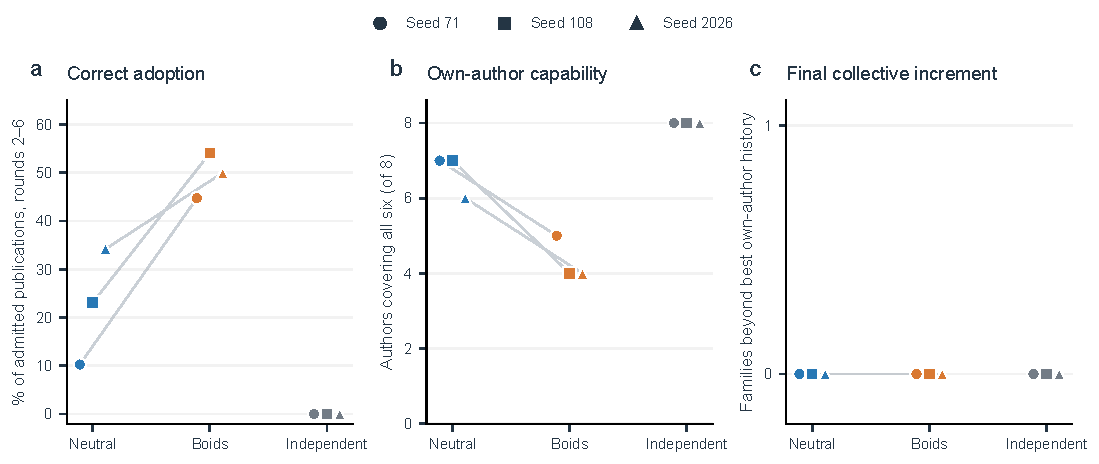
\includegraphics[width=\textwidth]{../../studies/tool_ecology/evidence/v031/analysis-02/figures/fig03-main-results.pdf}\caption{三个核心结果}\end{figure}
\section{对外能力相同，维护能力的位置不同}
所有作者最终通过自己的包及依赖，都能提供六类服务。因此累计服务集合 Jaccard 都等于 1。这不代表所有程序相同，也不代表社会内部没有变化。这个指标只看“能对外提供哪几类服务”。

把外部依赖剔除后，中性组自足六类作者为 7、7、6；Boids 为 5、4、4；独立组都是 8。换句话说，Boids 的 24 个作者历史中，有 11 个需要靠外部依赖补齐类别，中性只有 4 个。Boids 组的作者更常选择使用邻居能力，而不是在自己的声明闭包内保留全部能力。

这可以叫依赖组织差异。称为互补专业分工还需要另一层证据：依赖他人的作者是否持续提供了别人不可替代的贡献，组合是否增加能力。当前结果没有达到这层。

\begin{figure}[H]\centering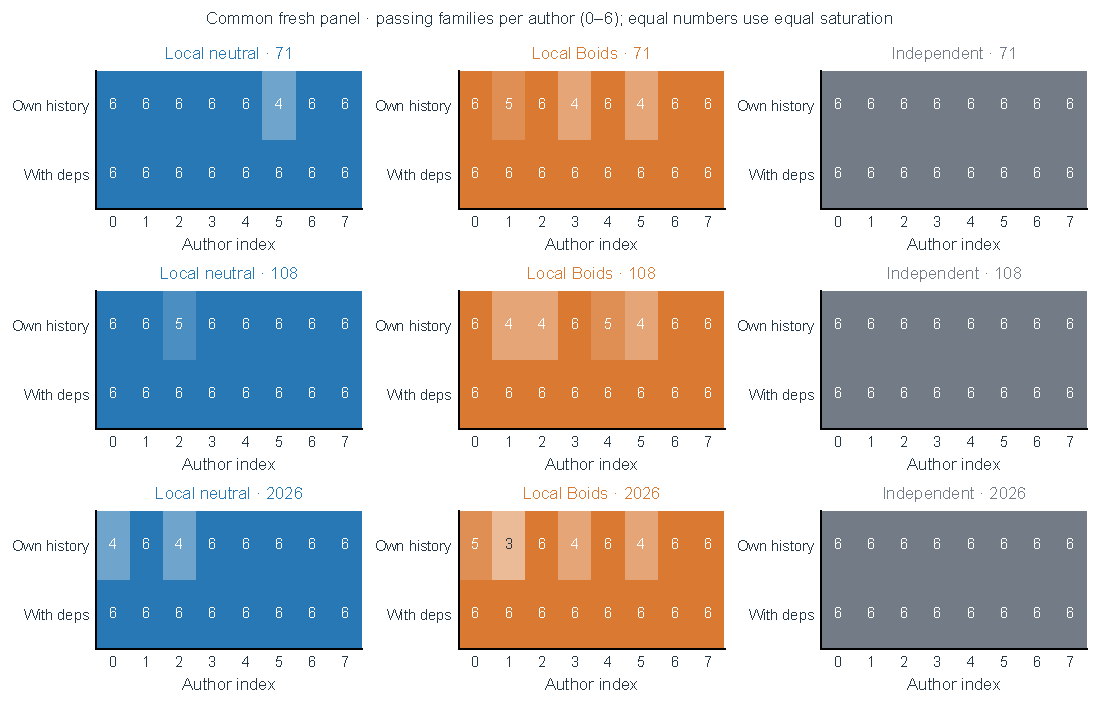
\includegraphics[width=\textwidth]{../../studies/tool_ecology/evidence/v031/analysis-02/figures/fig05-author-provenance.pdf}\caption{全部作者的自足与依赖能力}\end{figure}
自足历史库是同一作者多个历史版本的并集，且每份版本的闭包只能包含该作者。它不证明原创、独立理解或从未参考邻居代码。源码复制后形成的自足包，在这个定义下仍然自足。

\section{时间顺序给了一个非常具体的解释边界}
共同新 DEV 面板上，所有社会最晚第二轮就覆盖六类。两组在第一轮有过群体比最佳作者多一类：seed71 中性、seed2026 Boids。当时尚未发生工具交换，差异来自并行生成的功能覆盖组合。第二轮之后，两组的差距都消失了；其余社会也没有后续历史覆盖增量。

因此，短暂互补覆盖不能自动算作局部交互产生的组织。一个无需通信的并行集合，也会因为不同人的错误位置不同，暂时拼出更完整的功能范围。这是当前记录能直接支持的时间顺序判断。

与此同时，Boids 的采用并没有随着覆盖饱和消失，而是继续出现。持续传播的主要对象已经是可用能力，而非尚未填补的类别。对最终覆盖为零的解释应包括这个指标上限。

\begin{figure}[H]\centering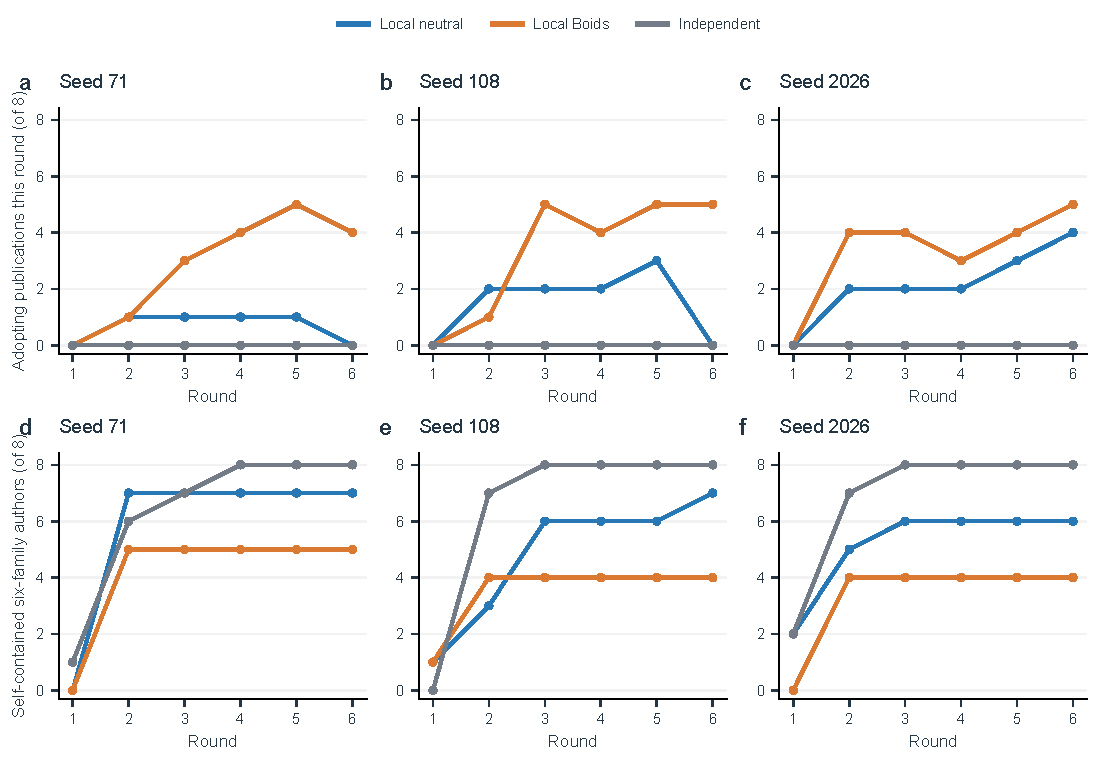
\includegraphics[width=\textwidth]{../../studies/tool_ecology/evidence/v031/analysis-02/figures/fig04-dynamics.pdf}\caption{逐种子动态}\end{figure}
\section{为什么“移除无损”不能等同于“协作没用”}
共同面板上九组群体覆盖都为六类，最佳自足作者历史也都是六类。72 次作者及其全部传递依赖移除，没有损失服务类别。用各作者最新已发布版本替代整个历史库计算，最终覆盖增量也全部为零。因此最终结果并非纯粹由历史版本并集掩盖。

但类别不变只是一个有限结论。删除后可能剩下更难维护、更慢或在其他数据上更脆弱的实现。这里没有模拟删除后的适应，也没有测出维护节省、执行成本优势或外部分布可靠性。我们能说“没有发现额外类别和类别上的不可替代贡献”，不能据此说一切协作价值都为零。

\section{窄化确实发生了，但维持方式值得细看}
420 份发布中，416 份声明全部六类；首轮 72 份全部声明六类。四份只声明 lookup 的发布都在 seed2026 Boids。三个完整通过，一份只过 1/6。没有一条原始轨迹满足“连续至少三轮、同一作者仅一类完整通过”的预设指标。

a00 第二轮借用邻居 lookup，第三轮通过自己的上一轮 wrapper 继续借用，两轮都 6/6。第四轮自己重写，只过 1/6；第五、六轮转回邻居整套工具的六类接口。a01 则只窄化一轮。

已有隔离诊断定位了第四轮程序的具体缺陷：计算了标准化 region，却没写回返回行。只补写回一行就从 1/6 变成 6/6。这个证据解释一份程序的失败，不是新实验，也不改变原始成绩。人工修复后的持续通过不能记作模型实际形成的角色。

\begin{figure}[H]\centering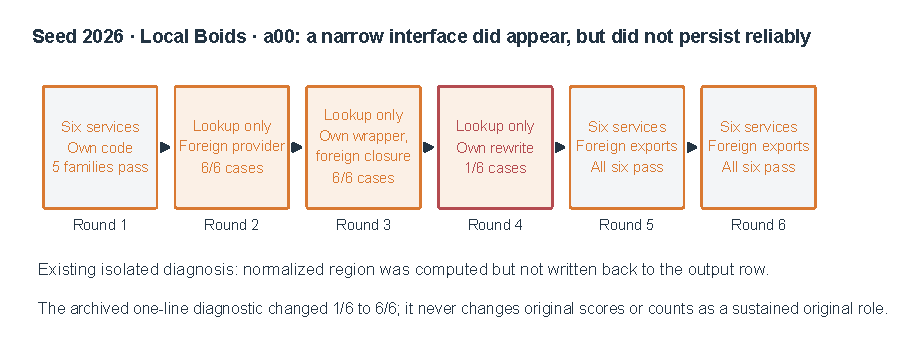
\includegraphics[width=\textwidth]{../../studies/tool_ecology/evidence/v031/analysis-02/figures/fig08-narrowing.pdf}\caption{窄化过程}\end{figure}
窄接口与窄专长也不同。这里早期 lookup 接口调用的邻居本身是通才库。它体现了接口选择，却没有证明只有该作者掌握了独立的 lookup 专长。

\section{大量采用表现为接口转发，不能把 wrapper 数当专业数}
新增静态检查只识别两种明确语法：声明检查直接从旧版本导入；或者函数只有一个 return，调用已经导入的函数。它不执行代码，不推断复杂 wrapper，也不把未识别语法自动判为原创。

在确有正确跨作者采用的发布里，中性 19/26、Boids 39/57 的全部声明检查都符合这两种接口转发形式。通才库被包上新版本、继续传播，足以产生大量真实执行边。

独立组也有很多旧版本接口转发，只不过作者相同。因此“wrapper 多”本身不是社会协作指标。必须同时看来自谁、是否实际执行、输出是否正确、提供的类别是否不可替代。

\Needspace{18\baselineskip}
\section{代码短了，是否就省钱了？}
根包 AST 节点的合并中位数为中性 822.5、Boids 114、独立 755。它只数新发布根包，不包含导入库；不是程序总复杂度或实际劳动量。逐社会的值变化很大，seed2026 中性和独立组的中位数都比 Boids 更小，不能拿合并中位数假装每个种子都同方向。

\begin{center}\small\resizebox{\textwidth}{!}{\begin{tabular}{lllll}\toprule
有效条件（三种子合计） & 模型调用 & 输入 tokens & 输出 tokens & 缓存输入 \\
\midrule
\textcolor{NeutralBlue}{局部中性} & 696 & 3,466,964 & 213,861 & 2,576,854 \\
\textcolor{BoidsOrange}{局部 Boids} & 661 & 3,317,264 & 205,653 & 2,399,887 \\
\textcolor{IndependentGray}{独立} & 695 & 2,470,848 & 206,737 & 1,803,280 \\
\bottomrule\end{tabular}}\end{center}
Boids 相对中性，调用少 5.0\%、输入少 4.3\%、输出少 3.8\%。相对独立组，Boids 输入多 34.3\%，输出只少 0.5\%。借用让提交的根包很短，却不保证交互过程同样短。看到更多邻居材料，仍然会消耗上下文。

这是实测资源描述，不是相同效能下的经济性结论。输入含缓存子集，价格没有核实；模型调用、tokens、代码体量和货币不能互相替代。

\begin{figure}[H]\centering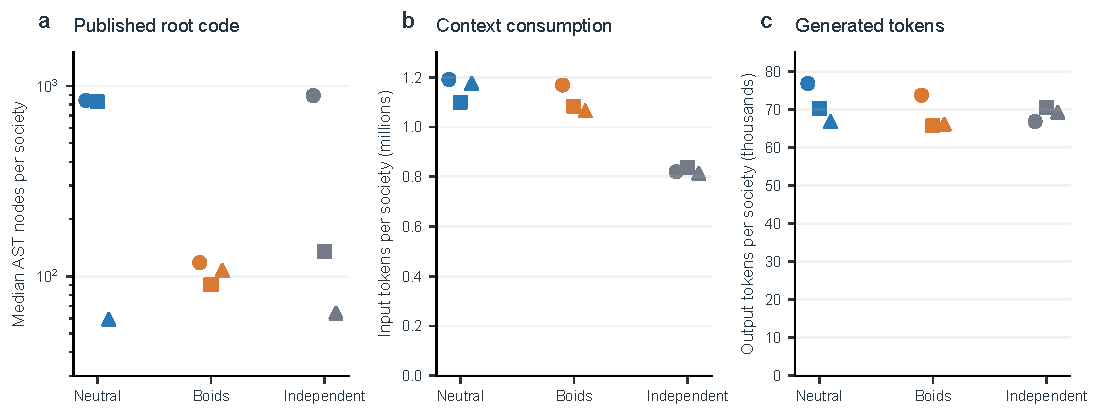
\includegraphics[width=\textwidth]{../../studies/tool_ecology/evidence/v031/analysis-02/figures/fig06-code-and-budget.pdf}\caption{代码体量与模型资源}\end{figure}
\section{正确率不支持一句话“Boids 更好或更差”}
在实际声明并被接收的服务案例上，中性 4,700/5,040（93.25\%）、Boids 4,598/4,884（94.14\%）、独立 4,840/5,076（95.35\%）。这是条件化的正确率，分母受服务声明影响。三组没有声明的服务不在这个分母里，也没有默认给窄发布补失败。

Boids 减中性的逐种子差为 +2.18、+2.36、-1.93 个百分点。合并均值略高不等于稳定提升，独立组更多六类全过也不等于已经证明单 agent 最优。两种简单概括都超过了当前证据。

15,000 个声明案例中，862 个失败。833 个只在 region 列不同，占失败案例约 96.6\%；其余是 revenue、units 或组合差异。三个条件都有 revenue 和 window 的失败。错误输出字段有助于定位契约边界，但相同字段可以由不同程序缺陷造成；只有已隔离的 a00\_r04 可以给出具体单行原因。

\begin{figure}[H]\centering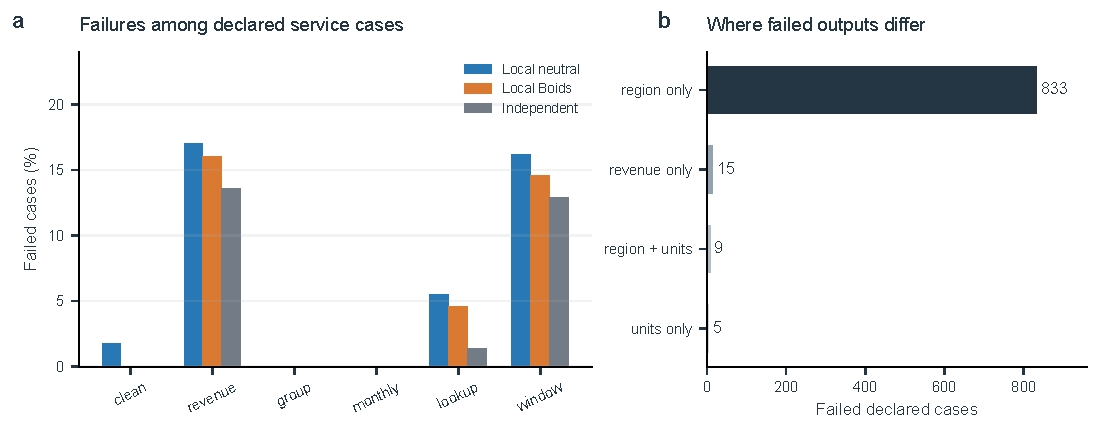
\includegraphics[width=\textwidth]{../../studies/tool_ecology/evidence/v031/analysis-02/figures/fig07-reliability.pdf}\caption{可靠性与输出差异}\end{figure}
\section{实际交互证据有多强}
420 份发布去掉追踪后，成绩全部一致。72 条预选“发布—边”干预记录，实际对应 70 个社会内唯一边；71 条记录、69 个唯一边有无崩溃的正确性丢失见证。重复出现在不同 root 下的内部边不重复算唯一边。

一个边未确认，因为唯一原本正确且命中的案例是空表，保持形状的返回扰动无法改变空列表。这是干预可识别性的限制；不能把它当作没执行，也不能从失败案例的变化反推必要贡献。该结果保留，没有另选更有利的边替换。

这些干预支持选定依赖在特定计算中确实影响结果。它们不证明社会没有替代工具，也不证明整个群体离不开对应作者。因此“单条调用有作用”和“移除作者不丢类别”完全可以同时成立。

\section{看网络，能说什么}
下面保留全部九个作者网络。箭头从 provider 指向 caller，按正确执行的版本对合并为唯一作者对；三个种子下中性有 2、3、4 对，Boids 有 7、6、8 对，独立为零。Boids 的采用涉及更多作者，并非只是一条边的案例重复。

这是执行网络，不是预先固定的 social ring。传递闭包可带来间接作者。作者投影可以有环，因为不同轮次可以互相借用；按版本展开的时间依赖图仍然无环。节点排列按固定作者编号，不是算法发现的社群，也不能据此肉眼宣布某种专业分工。

\begin{figure}[H]\centering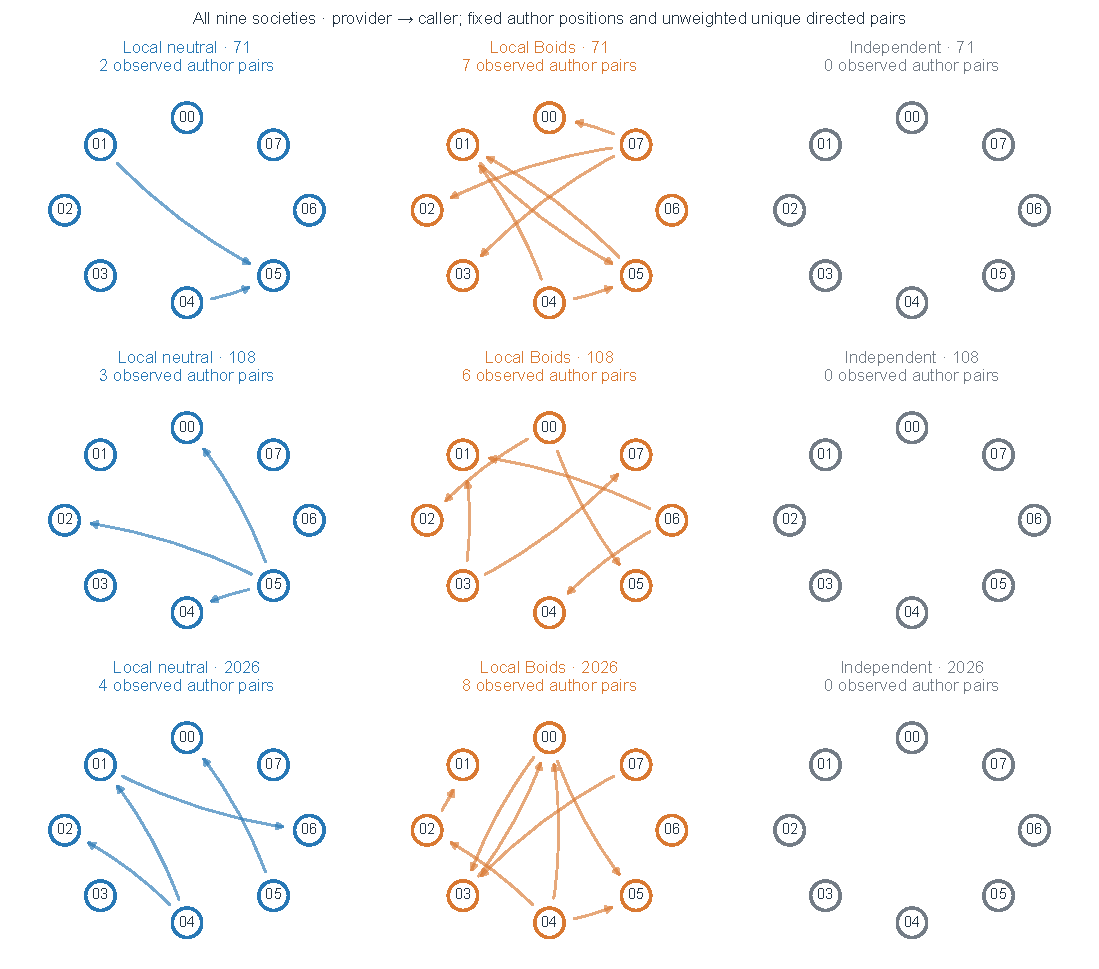
\includegraphics[width=\textwidth]{../../studies/tool_ecology/evidence/v031/analysis-02/figures/fig09-author-networks.pdf}\caption{全部九个社会的作者网络}\end{figure}
\begin{figure}[H]\centering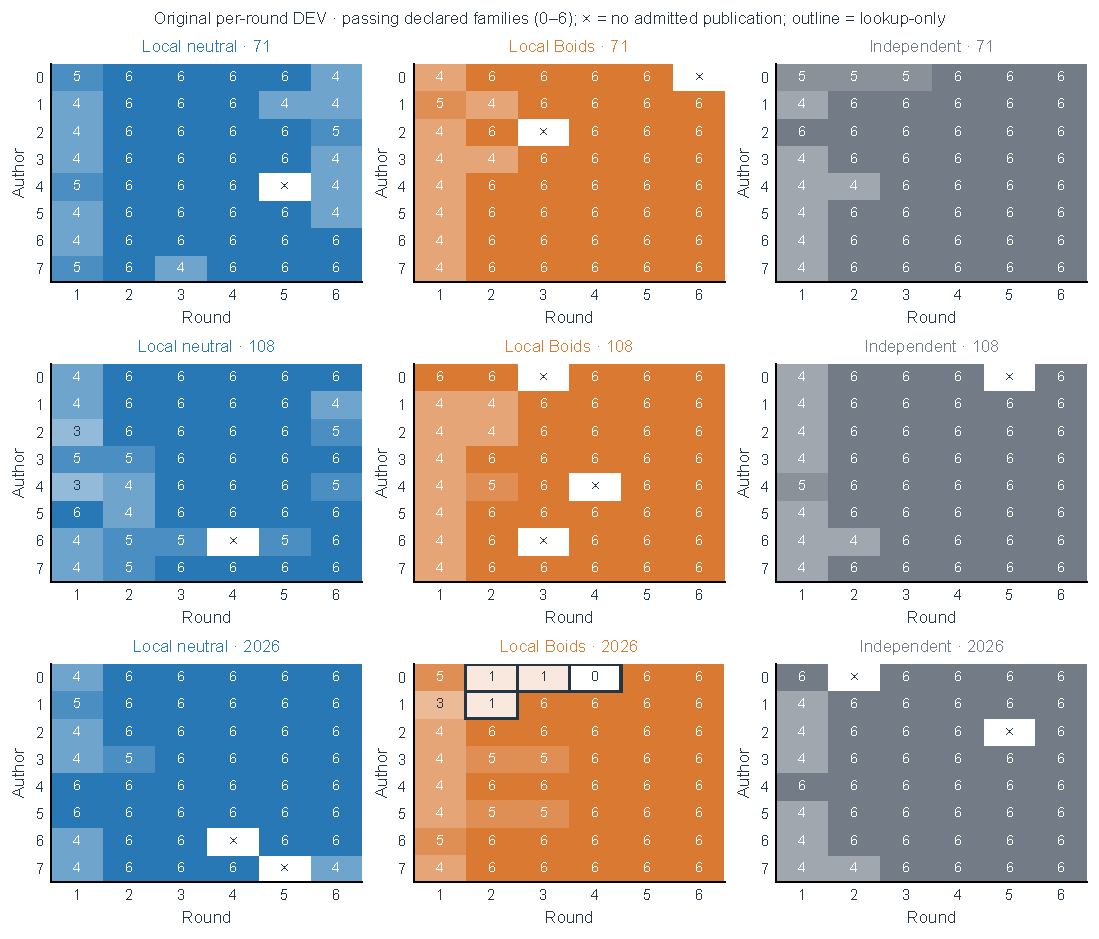
\includegraphics[width=\textwidth]{../../studies/tool_ecology/evidence/v031/analysis-02/figures/fig10-publication-breadth.pdf}\caption{全部发布机会的功能宽度}\end{figure}
\section{对 Boids 迁移本身的解释}
物理 separation 让个体避免空间碰撞；这里的 separation 提示可以通过“不重复造、直接借用”满足。alignment 同时鼓励复用可靠接口。于是二者在工具场景里可能共同推动通才库传播，而非把作者推向不同功能位置。这是与观测一致的机制解释，尚未用单独规则消融或中介干预识别。

工具还有持久性。早期完整实现不会像瞬时运动那样消失，后来很多作者都能围绕同一份库提供接口。依赖增加时，对外功能反而趋同。这解释了为什么“作者服务集合一样”和“维护能力位置不同”会同时出现。

本任务的共同需求是外部规定且保持不变的六类。没有需求漂移，没有资源制度迫使个体只能维护一部分，也没有发现新的共同目标。一个作者最晚第二轮就能覆盖全部需求，说明当前设置缺乏已证实的分工必要性。任务对通才较便宜、互补压力不足，是设计假设，不是已经证明的因果定律。

\section{对论文 story 的具体处理}
全文应围绕用户提出的核心问题：Boids 的简单局部规则，能否帮助理解 LLM 群体如何组织；迁移到认知贡献之后，哪些部分成立、哪些没有成立。

本轮成立的部分是：工具作为持久媒介允许追踪和干预；局部提示条件下出现更多正确采用；对外覆盖相同的作者，背后可以有不同依赖组织。本轮没有建立的部分是：稳定独立专长、必要的互补覆盖、超越单 agent 或集中分工的效能、对未见外部分布的优势。

因此本文的贡献是一个能拆开观察层级的研究框架，以及一个具体的边界结果。不能把“复用更多”改写成“涌现专业分工”，也不能把“覆盖增量零”写成“Boids 没用”。这里没有必要为了标题正面而继续花钱找胜利。

\section{来源、失败和分析边界}
本集合由修正 batch02 的五个完整社会及四个全新恢复社会组成。原 batch02 保留 ABORTED，不写入补跑；原测量作废 batch01 不进入比较。每个社会披露生成 revision 和 55/180 秒等待。有效九组 2,052 次调用，加超时部分 69 次，共 2,121。已知输入 9,480,041、输出 653,107、缓存输入 6,941,263；一次超时的服务商用量与账单未知。早期工程 107 次、测量作废 581 次单独保存。

新分析没有调用模型、grader，也没有重新运行程序或修复。它只对既有数据进行统计、可视化和解释。新的发布级采用率、静态语法分类、共同面板历史轨迹和 latest-version 对比均明确属于后验描述。所有种子、失败和不利结果都保留。

小样本、同质模型、六轮短期过程、有限 DEV、恢复选择、软提示规则、缺少单 agent/集中分工对照，都限制结论。当前可发表的讨论必须保留这些边界，不能把多个相关案例包装成大量独立社会。

完整源数据见 \href{https://github.com/xisen-w/boids-evolution/blob/codex/tool-ecology-dynamics/studies/tool_ecology/evidence/v031/analysis-02/README.md}{analysis-02}，英文全文见 \href{https://github.com/xisen-w/boids-evolution/blob/codex/tool-ecology-dynamics/paper/tool-ecology/main.pdf}{AAMAS 工作稿}。后续只分析现有证据，付费实验保持结束、自动实验跟进保持暂停。

\end{document}
